\documentclass[conference]{IEEEtran}
\usepackage{cite}
\usepackage{amsmath,amssymb,amsfonts}
\usepackage{algorithmic}
\usepackage{graphicx}
\usepackage{textcomp}
\usepackage{xcolor}

\def\BibTeX{{\rm B\kern-.05em{\sc i\kern-.025em b}\kern-.08em
    T\kern-.1667em\lower.7ex\hbox{E}\kern-.125emX}}
\begin{document}

\title{Voting Mechanisms in Reinforcement Learning}

\author{\IEEEauthorblockN{Jost Alemann}
\IEEEauthorblockA{\textit{Institute of Intelligent \& Cooperating Systems} \\
\textit{Otto von Guericke University}\\
Magdeburg, Germany \\
jost.alemann@ovgu.de}
}

\maketitle

% Research questions:
    % How voting can be incorporated inside multi-agent reinforcement learning algorithms?
    % What are the benefits?
    % Which voting mechanisms are used?

%ABSTRACT
\begin{abstract}
This paper aims to deliver an overview of how voting mechanisms can be incorporated in reinforcement learning.
Voting mechanisms and their properties are first introduced to the reader and then explained in more detail by describing their application in the field of multi-agent systems and reinforcement learning.
Additionally advantages resulting from the incorporation of voting mechanisms in reinforcement learning systems are concluded as they are shown in related work.
\end{abstract}

\begin{IEEEkeywords}
voting, reinforcement learning, multi-agent systems
\end{IEEEkeywords}

% INTRODUCTION
    % Motivation – Why is our research interesting
    % Problem – Where is a lack of knowledge
    % Idea – What solution do you present
    % Outline – How do you explain your insight
\section{Introduction}
In a democratic society choices are not made by a dictator but by taking the preferences of the whole society into account. Therefore each member of the society is entitled to cast a vote which represents it's preferences. Votes are then evaluated and a decision is derived by a given voting scheme. Plurality where the choice with the most votes wins, might be the most common voting scheme. Still there are many different voting schemes each of which can or cannot fulfil certain properties. This lies mainly in the subject of social choice theory and therefore is only described briefly if needed in the following.
\newline
The concept of considering multiple individuals' preferences by using a voting mechanism to make choices can be transferred to multi-agent reinforcement learning systems. This is motivated by the expectation that agents combine their limited perception and knowledge of the environment by deciding together. Therefore they are expected to obtain better results than agents that choose actions based on only their own perception \cite{partalas2008hybrid}.
\newline
Since learning agents try to optimise their own reward, they might learn to act selfish\cite{carr2008peer} or even learn to use strategic voting to exploit the voting system\cite{pitt2006voting} for that purpose.
Thus the design of a voting mechanism incorporated in a multi-agent reinforcement learning system is non-trivial.
To avoid extensive selfish behaviour in agents several constraints can be introduced by modifying the reward function or voting system.
The possibility to exploit a voting system depends on the chosen voting scheme.
Unfortunately Arrow's Impossibility Theorem implies that no voting scheme can be designed to be completely fair. This means there is always a way in which agents could exploit such a voting scheme by finding a certain voting strategy. Arrow's Impossibility Theorem will be explained later on in Section \ref{2BasicPrinciples}.
\newline
To give an overview over voting schemes and their possible properties Section \ref{2BasicPrinciples} introduces basic principles of social choice theory as far as they are required to understand the concepts described later on.
Section \ref{3RelatedWork} then shows related work to give example  applications of voting mechanisms incorporated in reinforcement learning.
Additionally used methods to avoid exploitation or selfish behaviour of agents will be highlighted.
As a conclusion different applications of voting mechanisms in multi-agent reinforcement learning settings are briefly compared in Section \ref{4Conclusion}.

% BASIC PRINCIPLES
    % Tell the readers about definitions, foundations that are used
\section{Basic Principles}\label{2BasicPrinciples}
The following text gives an introduction to basic principles of social choice theory that are needed to understand the concepts described in Section \ref{3RelatedWork}.
% Voting Schemes
\subsection{Different Voting Schemes}
To discuss properties of voting systems we have to introduce those systems first.
\begin{itemize}
    \item \textit{Plurality vote}:\\
    Voting scheme in which each voter is allowed to cast a constant number of votes and the alternative with the most votes is chosen.

    \item \textit{Majority rule}:\\
    Voting scheme that extends the Plurality vote voting scheme. The alternative with the most votes is chosen only if it also receives the majority of the total votes (i.e. if it also receives more than $50\%$ of the total votes). For voting scenarios with just two alternatives this is the same as Plurality vote. For voting scenarios with more than two alternatives, the alternative with the most votes could receive less than $50\%$ of the total votes. In this case no alternative is chosen or another decision making process is initialised (e.g. random choice or default case).

    \item \textit{Borda Count}:\\
    Voting scheme in which all alternatives are ranked by each voter. Each vote consists of the ranked list of alternatives and a corresponding score for each ranked alternative. Let $n$ be the total number of alternatives and let $r$ be the assigned rank of an alternative in a single vote (highest rank is one, lowest is $n$). The score is then calculated by \eqref{eq:BordaCount}.
    \begin{equation}\label{eq:BordaCount}
        score_{alternative}=n-(r_{alternative}-1)
    \end{equation}
    Each alternative gets a total score by adding up it's scores of each vote. This way higher ranked alternatives get a higher score per vote and alternatives that are more often ranked high receive a higher total score. At the end the alternative with the highest total score is chosen.
\end{itemize}

% Properties of Voting Schemes
\subsection{Properties of Voting Schemes}
\begin{itemize}
    \item \textit{Pareto efficiency}:\\
    If every voter prefers option X over option Y, then the society prefers X over Y.
    \item \textit{Independence of irrelevant alternatives}:\\
    If every voter prefers option X over option Y and option Z is removed without changing the former relation, the societies preference of X over Y also remains unchanged.
    \item \textit{Non-dictatorship}:\\
    No single voter possesses the power to always determine the group's preference.
\end{itemize}

% Arrow's Impossibility Theorem
\subsection{Theorems}
\begin{itemize}
    \item \textit{Arrow's Impossibility Theorem}\cite{arrow2012social}:\\
    Arrow's Impossibility Theorem states that no rank-order voting scheme can fulfil the properties Pareto efficiency, independence of irrelevant alternatives and non-dictatorship at the same time.
    Meaning that every voting scheme can be exploited by strategic voting \cite{pitt2006voting}. Voting not for the alternative that one prefers but another alternative to increase the chances that the preferred alternative is chosen at the end would be a simple example for strategic voting exploitation. Strategic voting highly depends on the given voting scheme and it's properties.
\end{itemize}


% RELATED WORK
    % How have other researchers tackled the problem
    % Outline benefits and downsides of other methods
    % Give a good structure to the current state of the art
\section{Related Work}\label{3RelatedWork}
\subsection{Voting and Social Constraints}
Carr et al. consider a multi-agent setting in their work \cite{carr2008peer} in which the environment has limited resources that are requested and later reallocated by the agents. All other agents then decide which proposals are accepted by voting to redistribute the global resources.
\newline
Each agent is considered to be capable of either responsible or selfish behaviour because of Arrow's Impossibility Theorem and the thereby implied possibility to manipulate the voting scheme by strategic voting. The authors point out that selfish behaviour is very likely in systems without social constraints.
Thus they add a reputation system consisting of each agent's voting history to the voting process. Responsible acting agents only vote for other agents with a responsible voting history. This works as a constraint for selfish behaviour because agents that always vote selfish will not be voted except by themselves and therefore receive no reward and eventually act responsible in the future.
\newline
The voting mechanism consists of two phases. In the first phase all agents vote on a threshold value $\tau$ that specifies how many votes a proposal requires to be accepted. A $\tau$ that is too low leads to many accepted requests and the global resource storage being bankrupted. On the other hand a $\tau$ that is too high leads to only few accepted requests and unsatisfied agents changing their strategy to get a reward in the future.
Threshold $\tau$ is decided in two rounds. In round one all agents propose a suggestion for value $\tau$. In round two all agents cast a vote for one of the two most common suggestions.
Resource reallocations are decided in phase two of the voting mechanism. First all agents propose a request or offer to the global resource storage. For simplicity reasons the authors only consider fixed value requests of resources. Then each agent votes on which proposal to accept. The authors found that a plurality voting scheme for the resource reallocation does not discourage selfish behaviour. To solve this the authors instead use a modified version of the Borda Count voting scheme which forces the agents to focus less on themselves but instead on the opinion on their neighbours. Equation \eqref{eq:ModifiedBordaCount} is a modified version of the Borda count equation \eqref{eq:BordaCount}.
\begin{equation}\label{eq:ModifiedBordaCount}
    score_{alternative}=\max(0,\ x-(r_{alternative}-1))
\end{equation}
Where $r$ again represents the number of the alternatives rank and $x$ is the number of responsible agents of the population. Selfish agents receive no Borda points from responsible agents' votes because responsible agents rank other responsible agents higher than selfish agents. As a result the reputation constraint which is represented by a voting history is used to reduce the Borda score of selfish agents even when they always rank themselves first.
\newline
The authors use Q-learning as reinforcement learning algorithm. In this system they only have two Q-values because there is only one state and the two actions behaving either responsible or acting selfish.
As a result the authors run simulations to show that responsible agents get more satisfaction than selfish acting agents. Therefore they initialise the Q-values so that the value for a responsible action is larger than the one for a selfish action. At a certain time step they then introduce selfish acting individuals to the population by adding agents whose Q-value for a selfish action is larger than the one for a responsible action. They observe whether the newly introduced selfish agents learn to act responsible or whether they stay selfish and monitor their satisfaction (i.e. a score representing whether an agent is successful in the system or not).
\newline
The authors show that selfish agents can either learn to adapt the responsible behaviour of the population and receive greater satisfaction or stay selfish and end up with a low satisfaction in the system. This means that their concept of adding reputation as a social constraint and modifying the voting scheme in a multi-agent reinforcement learning setting can ensure that agents learn to not manipulate a voting mechanism by strategical voting for their own purposes but to cooperate with other agents by voting in a responsible manner. Some results of Carr et al. \cite{carr2008peer} can be seen in Fig. \ref{SelfishVSResponsibleAgents}.

\begin{figure}[bt]
    \centering
    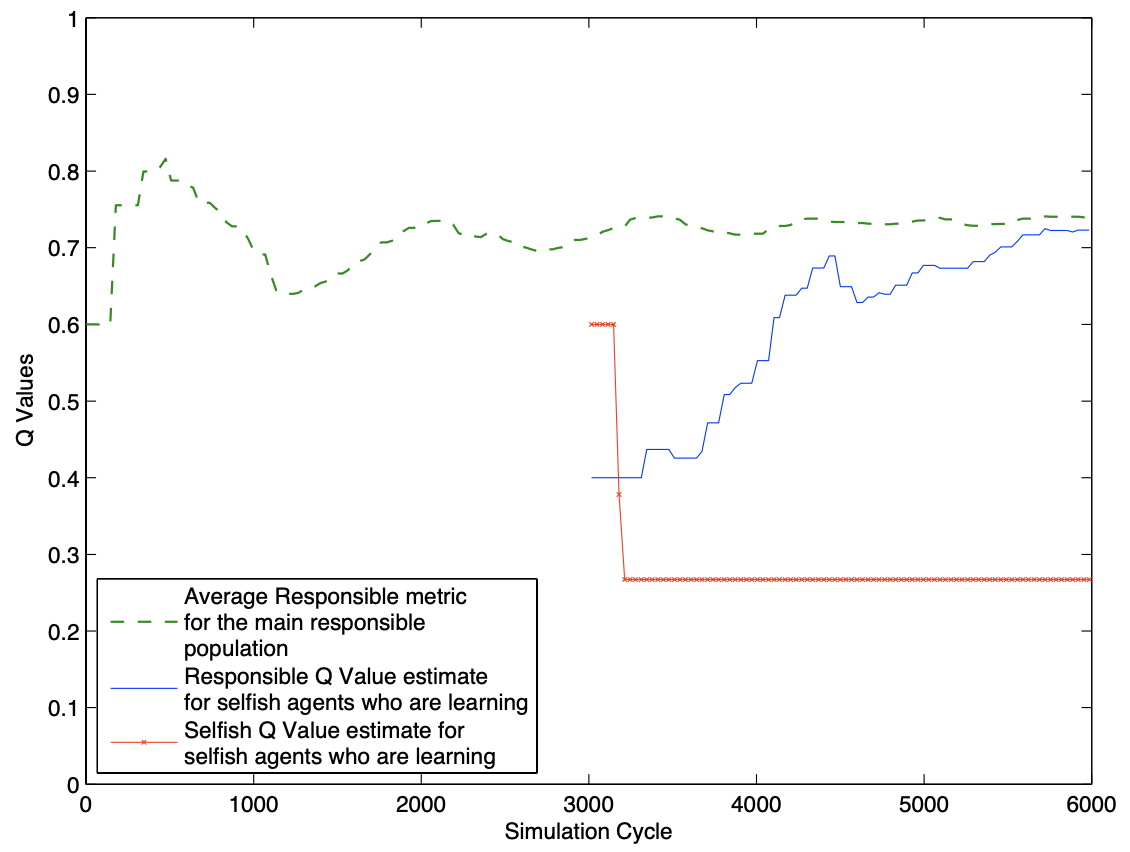
\includegraphics[width=0.45\textwidth]{Qvalues.png}
    \caption{Q Value estimates of the Responsible Agents and the initially Selfish Agents}
    \label{SelfishVSResponsibleAgents}
\end{figure}

\subsection{Voting and Multi-Agent Strategies}
A different setting and concept for the use of voting mechanisms in reinforcement learning is explained in the work of Partalas et al. \cite{partalas2008hybrid}. They consider a multi-agent setting in which the agents are predators that learn to catch a prey.
\newline
Additionally they introduce strategies which are combinations of high level actions assigned to an individual agent. An example named by the authors that would fit into the setting would be that one predator moves closer to the prey while another agent stays near the prey. It should be noted that as far as this work goes, strategies have to be designed manually and that their quality might heavily influence the performance of the agents.
\newline
If multiple predators are cooperating to catch the prey they do not choose an action individually but instead vote for a strategy that is then executed by all agents. The agents generally use majority rule as the voting scheme to decide on which strategy follow. This results in the difficulty that in settings where only a small number of predators cooperate there is only a small probability that a strategy receives the majority of votes. The authors tackle this problem with choosing a rank-based voting scheme instead. All predators rank the strategies based on their corresponding Q-value where the largest Q-values are ranked better and smaller Q-values receive worse ranks. The ranks of each agent's ranking are averaged so that each strategy receives a total ranking score. Since rank one would represents the largest Q-value in a ranking, the strategy with the lowest average ranking score will be chosen. Another criterion has to be defined which decides on a single strategy if multiple strategies tie by both receiving the lowest average ranking score. For example the predators rankings could be weighted based on each predator's distance to the prey. In this case predators that are near to the prey would receive a lower weight than distant predators because the smallest value is chosen.
\newline
This work does not use reputation or another social constraint to discourage agents from manipulating the voting scheme by strategic voting like the work discussed before. Such a constraint is not required in this work because each predator agent is encouraged to cooperate with other predators by giving each predator the same reward. In this case a selfish acting predator agent is also an agent that cooperates with other predator agents. To heavily encourage predators to cooperate and to vote on and use strategies the authors chose to add a different constraint. Only cooperating predators receive a reward whenever the prey is caught. Predators that act individually are not rewarded.
\newline
As a result it is essential to define a mechanism that specifies whether agents are cooperating and which agents cooperate with which other agents. The authors state that this mechanism again has to be chosen per setting. As an example in the considered predator-prey setting cooperating groups of agents could be chosen by distance to the prey.
\newline
The authors expect predators that learn to vote on strategies which they execute perform better than individual learning predators. They compare an independent learners approach, the voting reinforcement learning approach and a hybrid of both approaches with each other.
The hybrid approach uses the Sparse Tabular Q-learning algorithm.
The individual learner approach as well as the voting reinforcement learning approach use Q-learning.
In the individual learner approach each agent learns it's own Q-values that are not shared with other agents. Also the agents are not taking actions executed by other agents into account.
In the voting reinforcement learning approach the agents instead learn own Q-values if they are not currently cooperating with other agents but are learning shared Q-values when they are in a cooperating group.
The performance of each approach is measured in the average time it takes the predators to catch the prey when using given reinforcement learning algorithm.
The authors also consider different board sizes and different numbers of predator agents. They show that the voting reinforcement learning approach performs better than the other approaches in each tested setting. Some results of Partalas et al. \cite{partalas2008hybrid} can be seen in Table \ref{table:AvgCaptureTimes}.

\begin{table}[tb]
    \centering
    \caption{Average capture times for different values of the predator and grid size parameters}
    \begin{tabular}{c c c c}
        \hline
        Predators & RL-Fusing & IL & STQ \\
        \hline
        3 & 10.17 & 17.26 & 13.49 \\
        4 & 7.81 & 13.24 & 13.01 \\
        5 & 6.7 & 10.77 & 10.16 \\
        \hline
        \\
        \hline
        Grid size & RL-Fusing & IL & STQ \\
        \hline
        10 & 7.28 & 11.62 & 10.5 \\
        12 & 10.17 & 17.26 & 13.49 \\
        14 & 14.05 & 22.79 & 22.04 \\
        \hline
    \end{tabular}
    \label{table:AvgCaptureTimes}
\end{table}

% CONCLUSION
\section{Conclusion}\label{4Conclusion}
The related work shows that voting mechanisms can be incorporated into multi-agent reinforcement learning settings. Although they show that this incorporation yields more design choices and also design difficulties for the reinforcement learning system, they also highlight the possible advantages of the use of voting mechanisms. Voting mechanisms can improve the performance of learning agents. They can also be used in combination with additional constraints to encourage or even enforce a certain learning direction for agents.

\bibliographystyle{IEEEtran}
\bibliography{refs}

\vspace{12pt}

\end{document}

